\section{Introduction}
\subsection{History of the study of the brain and neuroscience}
It was thought in the Late Middle Kingdom era (2040-1782BC) that the heart was the holder of intelligence, given that in preparation for mummification, the brain was removed; hence to learn something by heart \cite{dintroduction}. By the fifth century BC it was the Pythagorean Alcmaeon of Croton who considered the brain to be where the mind was located \cite{inbook}. This was then taken further when Hippocrates believed the brain to be the seat of intelligence \cite{finger2001origins}. Over the next 2000 years, through dissection, more and more parts of the brain were being discovered. 

Leaping forward to the first half of the $19^{th}$ century, we get a variety of discoveries  involving electrical currents and the brain. This led to the discovery in the middle of the $19^{th}$ century that neurons were electrically excitable and that the activity of these neurons instigated a change in the electrical state of adjacent neurons \cite{2013}. During the second half of the $19^{th}$ century, we had discoveries of the connection between the brain regions and sensory and motor functions. In particular, we look at the somatosensory region, which accounts for things like sense of touch and perception \cite{2005}. 

The somatosensory cortex contains many columns. Each column contains 6 layers, although in some instances, this can be 4, though we do not discuss these here. These layers reach from the higher cortical layers, namely, 1 and 2, through to the deeper cortical layers of 5 and 6. It is one of these cortical columns that we take our focus on and describe in more detail in the next section \cite{Reimann_2017}.
\begin{figure}[H]
\begin{center}
\captionsetup{justification=centering}
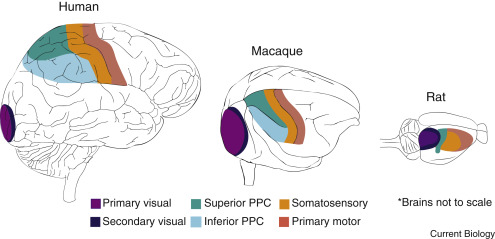
\includegraphics[width=12cm]{graph/brain.jpg}
\caption{Regions of the brain  \cite{Whitlock2017PosteriorPC}}
\end{center}
\end{figure}
\subsection{Blue Brain Project (BBP)}
The Blue Brain Project was founded in May 2005 with the initial goal of creating a simulation of the rat neocortical column. In October of 2015, after various experimentations involving the brain \cite{2013}, the BBP created a first draft of a reconstruction of the neocortical microcircuitry in the somatosensory cortex in a juvenile rat \cite{2015}. This reconstruction contained approximately $31,000$ neurons, where, through patch-clamp studies, there were 55 layer-specific morphological and 207 morpho-electrical neuron sub-types. Through the digital reconstruction, where neurons are positioned according to a restriction to biological bouton densities and number of synapses per connection, their overlapping arbors form approximately 8 million connections from around 37 million synapses \cite{2015}. 

From the BBP website on the construction of the neocortical column, we have results whereupon there are 35 instantiations of a biologically correct model that have been produced. That is, we have 5 rats, with 7 instantiations each, from which there are a further 7 instantiations that take the average of each of the instantiations of the 5 measured rats. We use the data representing the final instantiation, that is labelled as Bio-M in their paper \cite{Reimann_2017}.
\begin{figure}[H]
\begin{center}
\captionsetup{justification=centering}
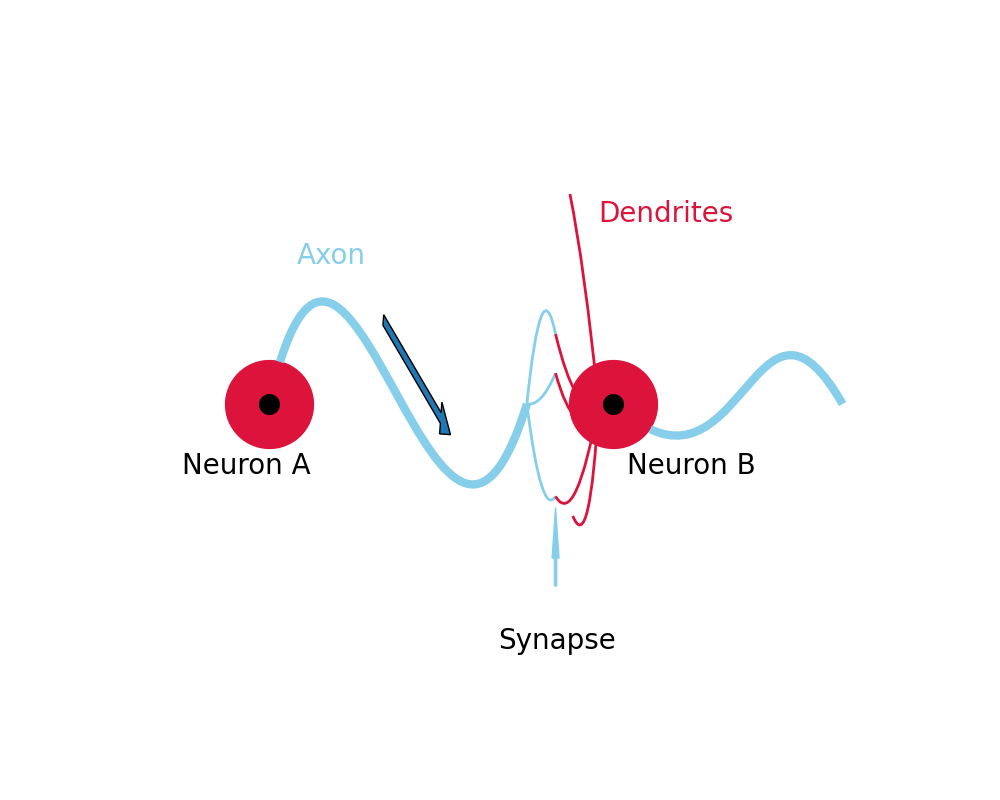
\includegraphics[width=12cm]{graph/cell.png}
\caption{Visual representation of a synaptic connection between two neurons}
\end{center}
\end{figure}
\subsection{Models}
We have four random graph models of the MC plus the \ER model that we wish to compare using topological statistics as to their accuracy in replicating the statistics from the biologically correct model produced by the BBP, the Bio-M MC. The first of these random graph models, is the Configuration model, $\mathcal{G}_{C}$, which rewires the connections between the neurons, without allowing for any self loops while also preserving the in and out degree of each neuron.
Our second random graph model, the Geometric Configuration model, $\mathcal{G}_{GC}$ is identical to the Configuration model while also taking into account the observed distances between connected neurons. 

The third random graph model, the Block Configuration model, $\mathcal{G}_{BC}$, extends the idea of the Configuration model by firstly subdividing the connectome into blocks on a layer by layer basis. We have 6 layers, whereby layers 2 and 3 are considered together. This accounts for 25 blocks. Within each block we have a subset of connected pairwise neurons of the connectome. Each block applies the same connection method as the Configuration model thereafter before being reassembled into a realisation of the connected random graph $\mathcal{G}_{BC}$.


In the final random graph model, the Block Geometric Configuration model, $\mathcal{G}_{BGC}$ we extend the ideas of the previous models,  $\mathcal{G}_{BC}$ and $\mathcal{G}_{GC}$, and combine them. That is to say, we again subdivide the connectome into blocks on the same basis as stated previously for the Block Configuration model, however, this time when we compute a permutation of the connected pairwise neurons in each subset, we take the added constraint of a distance-dependence. Upon completion of a rewiring of each block, we can reassemble the blocks, much like the Block Configuration model, to obtain a realisation of the random graph model $\mathcal{G}_{BGC}$. 




